% Chapter Template

\chapter{Results - Rubik's Cube} % Main chapter title

\label{sec:ResRubiks} % Change X to a consecutive number; for referencing this chapter elsewhere, use \ref{ChapterX}

%----------------------------------------------------------------------------------------
%	SECTION 1
%----------------------------------------------------------------------------------------

In this second results section, I discuss my experiments on the Rubik's cube. I have run reasonably comprehensive experiments on the 2x2x2, throwing 6 of my solvers at the problem. As mentioned in \ref{sec:Puzzles}, the 2x2x2 \textbf{RC}, in spite of its deceivingly simple physical appearance, is actually not that much easier to solve (by hand) than the 3x3x3. For instance, it takes me usually just under 1 minute, wherras the 3x3x3 takes me only double that time, just under 2 minutes. I am obviously a beginner in Rubik's cube handsolving, but my personal ratio of time-to-solve and perceived difficulty is in line with that of experienced speedcubers who might take and average of, say, 2-3 seconds for the 2x2x2 and 10 seconds for the 3x3x3.
\\
Computing wise, the 2x2x2 was of decent size for my purpose, with its 88 million configurations. Let me start with a table summarizing which solvers I have attempted to run on the 2 dimensions I have attempted to experiment with:

\begin{center}
\begin{tabular}{l*{5}{c}r}
\hline
\textbf{solver}      & & \textbf{Rubik's} & \textbf{2x2x2} & \textbf{3x3x3} \\
\hline
BFS   &   &        &  x  &  x  \\
\hline
Kociemba   &   &      &  x  &  x  \\
\hline
A$^{*}$[Kociemba]  &   &  &  x  &  x  \\
\hline
A$^{*}$[DL[A$^{*}$[Kociemba]]]  &   &  &  x  &  x  \\
\hline
A$^{*}$[DRL]  &   &  &  x  &  \\
\hline
A$^{*}$[DQL]  &   &  &  x  &  \\
\hline
%MCTS[DQL][c=0]  &   &  & x &  \\
%\hline
%MCTS[DQL][c=69]  &   & & x &  \\
%\hline
\end{tabular}
\end{center}








\Section{2x2x2}
All the following experiments on the 2x2x2 \textbf{RC} have been run using my Solver's \textit{performance\_test} (see \ref{sec:codesolvers}): for each level of difficulty, the test present the solvers with the same 100 random configurations (for fairness and to increase the significance of the results). The levels of difficulty (number of scrambles from goal) used here go from 2 to 20 in step of 2. The tests were also run with perfect shuffling (difficulty = $\infty$ on the graphs), corresponding to taking scrambling to $\infty$ as explained in \ref{Theory:222RCSSS}).

\Subsection{BFS}
BFS is the only one for which I used a step of 1 on the difficuly and stopped at 5 as it was clear it would not go any further. Given that the run time and expanded nodes are clearly going to increase linearly, and given where 5 scrambling from goal took this solver already, there was no point going any further!

\Subsection{Kociemba, A$^{*}$[Kociemba], A$^{*}$[DL[A$^{*}$[Kociemba]]]}
Next, let me discuss Kociemba (see \cite{HKociemba} and \cite{Kociemba}) and associated experiments. We obviously expect Kociemba to be by far the fastest solver since it is handcrafted with much specific knowledge about the Rubik's cube group theory and multi-stage solving which I discussed in \ref{Theory:RCMSS}. I found the 2x2x2 library I used to not be optimal however, despite claims to the contrary. I have not had the time to investigate why this was not the case, but empirically I found that for instance running A$^{*}$ with Kociemba's cost as a heuristic was resulting in higher quality (i.e. of lower cost) solutions, clearly showing the non-optimality of Kociemba to begin with.
\\
\noindent Similarly to the higher dimensions \textbf{SP} from the previous section, there was no hope for me to run a perfect solver on the 2x2x2 \textbf{RC}. For starter, I have no admissible heuristic to guarantee optimality! Even if I had found one such heuristic and managed to implement it, it is doubtful I could have solved all 88 millions configurations without considerable work and time to reduce the configurations via symmetry arguments. As a result, I used solutions from A$^{*}$[Kociemba] on (perfectly) randomly generated configurations to train my \textbf{DL} heuristic. Thinking of it, it is rather amusing since Kociemba is itself using a two-stage IDA$^{*}$ solver, so I end-up here with 3 levels of nested A$^{*}$ algorithms, namely A$^{*}$[DL[A$^{*}$[IDA$^{*}$[2-stage-subgroups]]]].
\\
Notice finally that, since I have no optimal solver for the \textbf{RC}, I have set Kociemba as my benchmark in the performance test for the purpose of computing the optimality score. This is why some (actually all) of the other solvers will show scores larger than 100\% (top-right graph of figure \ref{fig:222RCPerformance}).






\Subsection{Deep Reinforcement Learner \& Deep Q Learner}
\label{sec:S33DRL}
To get my \textbf{DRL} and \textbf{DQL} heuristics, I have run the DeepReinforcementLearner and DeepQLearner with the following main parameters:
\begin{itemize}
\item Update the target network every 1,000 epochs (\textit{update\_target\_network\_frequency=1000}) or when the MSE falls below 10 basis points of the maximum target cost-to-go (\textit{update\_target\_network\_threshold=1e-3})
\item Run for a maximum of 11,000 epochs (\textit{nb\_epochs=11000}) or when the maximum target so far has not been increasing by more than 1\% in the last 5,500 epochs (\textit{max\_target\_uptick=1e-2} and \textit{max\_target\_not\_increasing\_epochs\_pct=0.5})
\item At every update of the target network (\textit{training\_data\_every\_epoch=False}), generate 10,00 sequences of puzzles (\textit{nb\_sequences=10,000}), each comprised of a 15-scramble puzzle back to goal state, with all intermediary puzzles along the path (\textit{nb\_shuffles=15}).
\item Use a fully connected network (\textit{network\_type=fully\_connected\_net}) with three hidden layers of size 600, 300, 100 (\textit{layers\_description=(600,300,100)}) and use torch.optim.RMSProp as optimiser (\textit{optimiser=rms\_prop}) with an exponential scheduler (\textit{scheduler=exponential\_scheduler}) with gamma 0.999 (\textit{gamma\_scheduler=0.9999}) and \textit{learning\_rate=0.001}. The networks architecture is shown in figure \ref{fig:222RCnets}.
\end{itemize}
Graphs \ref{fig:222RCDRL} and \ref{fig:222RCDQL} show both learners' following metrics tracked over the epochs:
\begin{itemize}
\item learning rate, which decreases due to the scheduler, but gets reset at each network update.
\item max target. One interesting dynamic during learning is that due to the way targets are constructed using value-iteration update, and starting from an all 0 network, the max target only increases by about 1 at best at every network update. That is, the first network only learns how to differentiate goal from non-goal, then the second one learns how to differentiate goals, cost 1 and cost 2+ \dots. This is why I have introduced the \textit{update\_target\_network\_threshold} discussed above. It makes sure we do not waste time initially training the left-hand-side network when training is easy. \textit{max\_target\_uptick} and \textit{max\_target\_not\_increasing\_epochs\_pct} on the other hand make sure that we stop training altogether when the max target does not grow anymore. This is because we do not know a-priori what the God number of a given puzzle/dimension is. Let us assume for the sake of the argument that it is 15: that means that beyond 15 updates of the target network we might not get much benefit to additional training and value-iterating.
\item the loss (MSE for \textbf{DRL}, MSE + CrossEntropyLoss for \textbf{DQL})
\item the loss divided by the max target. The exit criterion \textit{update\_target\_network\_threshold} is based on that quantity, since a loss of e.g. 0.01 means little if the we do not compare it to the possible range that the cost-to-go can take.
\item The percentage of all the possible puzzles of that dimension \textit{seen} by the learner. This is an interesting quantity, as it tells us how well the solvers are able to generalise. From both graphs (\ref{fig:222RCDRL} \& \ref{fig:222RCDQL}) we can see that the learners saw less than 1\% of all puzzles. It is good to keep in mind however that \textit{seen} does not mean really much here, since the learning is \textit{unsupervised}. This is quite in contrast to the DeepLearner, whose traiing data consist of puzzles with their cost-to-go computed by a \textit{teacher} (optimal or other efficient solver).
\end{itemize}


\begin{figure}
  \noindent
  \makebox[\textwidth]{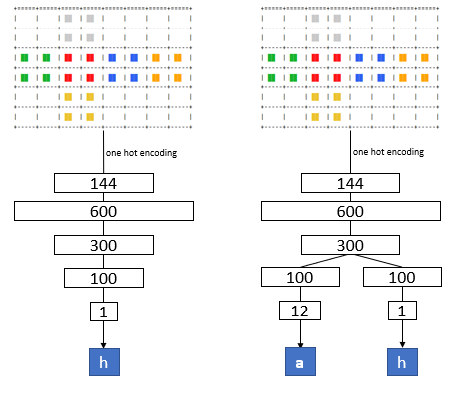
\includegraphics[scale=0.6]{./Figures/222RCnets}}
  \caption[222RCnets]{2x2x2 \textbf{RC} architecture for \textbf{DRL} (left) \& \textbf{DQL} (right) heuristics training}
  \label{fig:222RCnets}
\end{figure}


\begin{figure}
  \noindent
  \makebox[\textwidth]{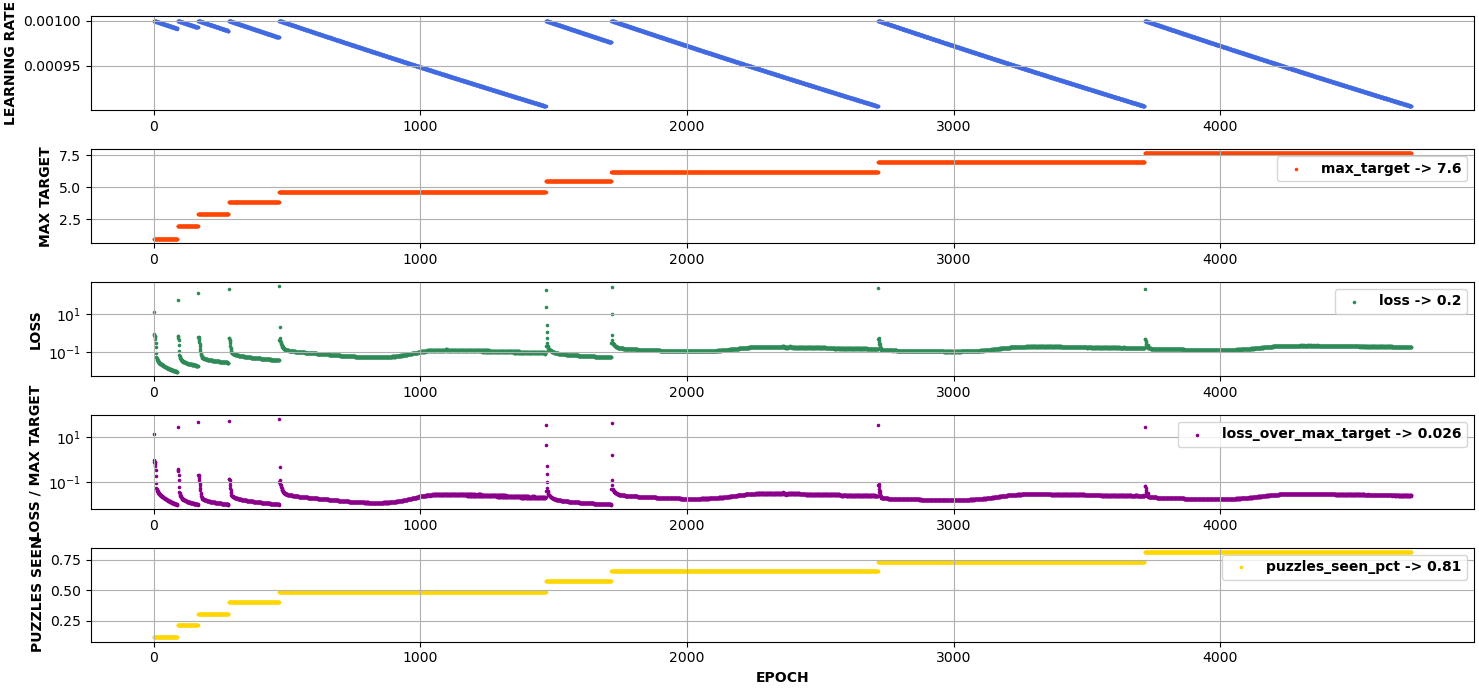
\includegraphics[scale=0.5]{./Figures//222RCDRL}}
  \caption[222RCDRL]{\textbf{DRL} of the 2x2x2 \textbf{RC}}
  \label{fig:222RCDRL}
\end{figure}

\begin{figure}
  \noindent
  \makebox[\textwidth]{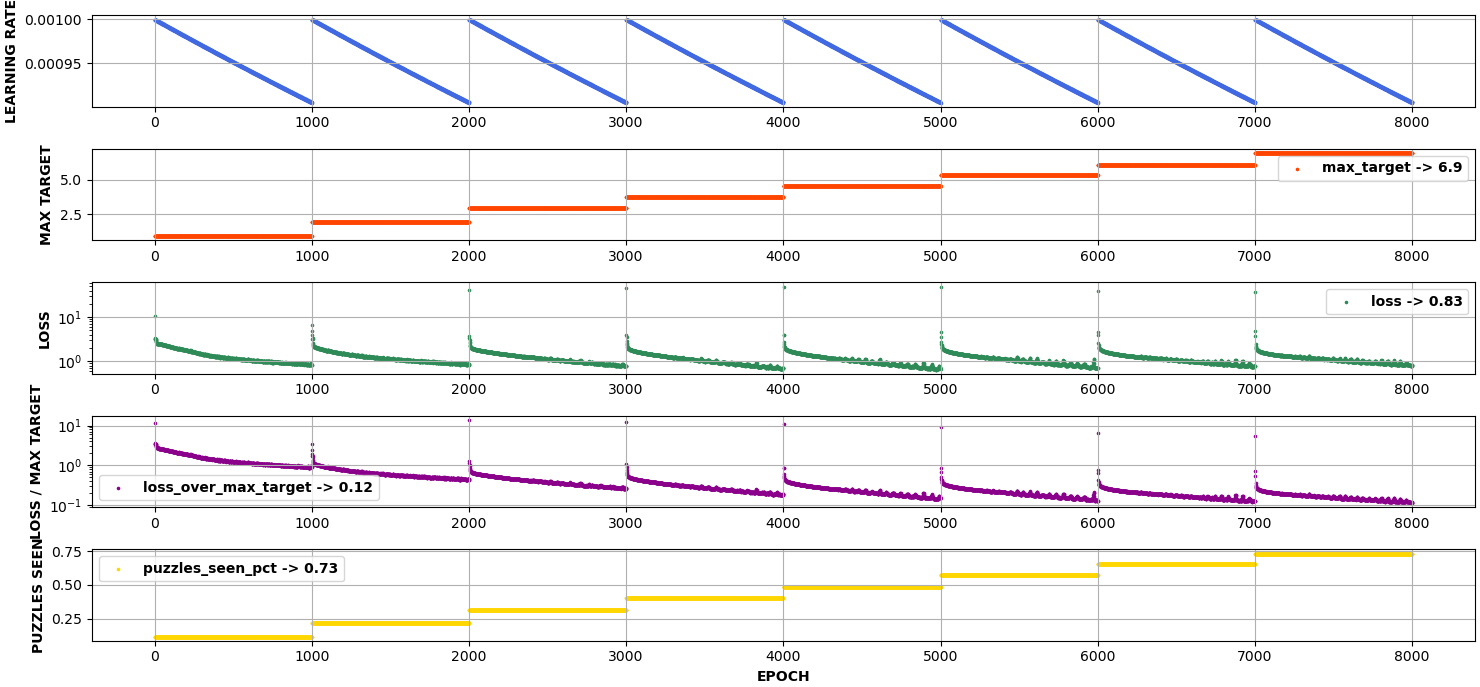
\includegraphics[scale=0.5]{./Figures//222RCDQL}}
  \caption[222RCDQL]{\textbf{DQL} of the 2x2x2 \textbf{RC}}
  \label{fig:222RCDQL}
\end{figure}




\Subsection{Solvers' comparison}

We summarize as usual the 2x2x2 \textbf{RC} performance tests by our usual metrics \ref{fig:222RCPerformance}. Overall, the \textbf{DL} and \textbf{DRL} managed to solve all cubes (though \textbf{DL} took over an houd and \textbf{DRL} up to 6 hours for the slowest cube they encountered. Both methods outperformed in terms of optimality score Kociemba and got on par with A$^{*}[Kociemba]$. Their max cost over all cubes encountered was 12 for up to 20 shuffles, and 13 for $\infty$ shuffling. Considering God's number for the 2x2x2 \textbf{RC} of 11, this is rather impressive!
\\
\\
An very interesting remark is that if we check the learning graph \ref{fig:222RCDRL} of the \textbf{DRL}, we can see it only ever assigned a cost-to-go (value function) of 7.6 at most. Despite that fact, it was still able to solve cubes requiring 13 moves. How is that possible? Notice that the loss of 0.2 towards which it converged at the end of its training is misleading, since it is not a loss versus the actual true cost-to-go, but rather versus that of the target network. My theory is that while the value the \textbf{DRL} assigned to hard-to-solve cubes is off (by at least 4 or 5), it is likely the case that the network gets the relative value of neighbouring cubes about right (given that the value-iteration teaches the solver that, it is not super surprising either), and this is sufficient to guide A$^{*}$ extremely well. If both the absolute value of the cost-to-go and the relative (among neighbouring cubes) was totally off, we would indeed not expect the heuristic to make A$^{*}$ any better than, say, \textbf{BFS} and we would therefore not expect it to be able to solve \textit{costly} cubes in 10-13 moves.
\\
\\
Finally, we can see that \textbf{DQL}, despite showing seemingly/visually cleaner and more monotonic loss convergence than \textbf{DRL} (see \ref{fig:222RCDQL} versus \ref{fig:222RCDRL}), struggled a lot more to solve difficult cubes (above 10 shuffles). Clearly this shows that my earlier findings on the 3x3 \textbf{SP} are likely not universal, and very much depend on the parameters set during training, as well as on the problem at hand.

\begin{figure}[H]
  \noindent
  \makebox[\textwidth]{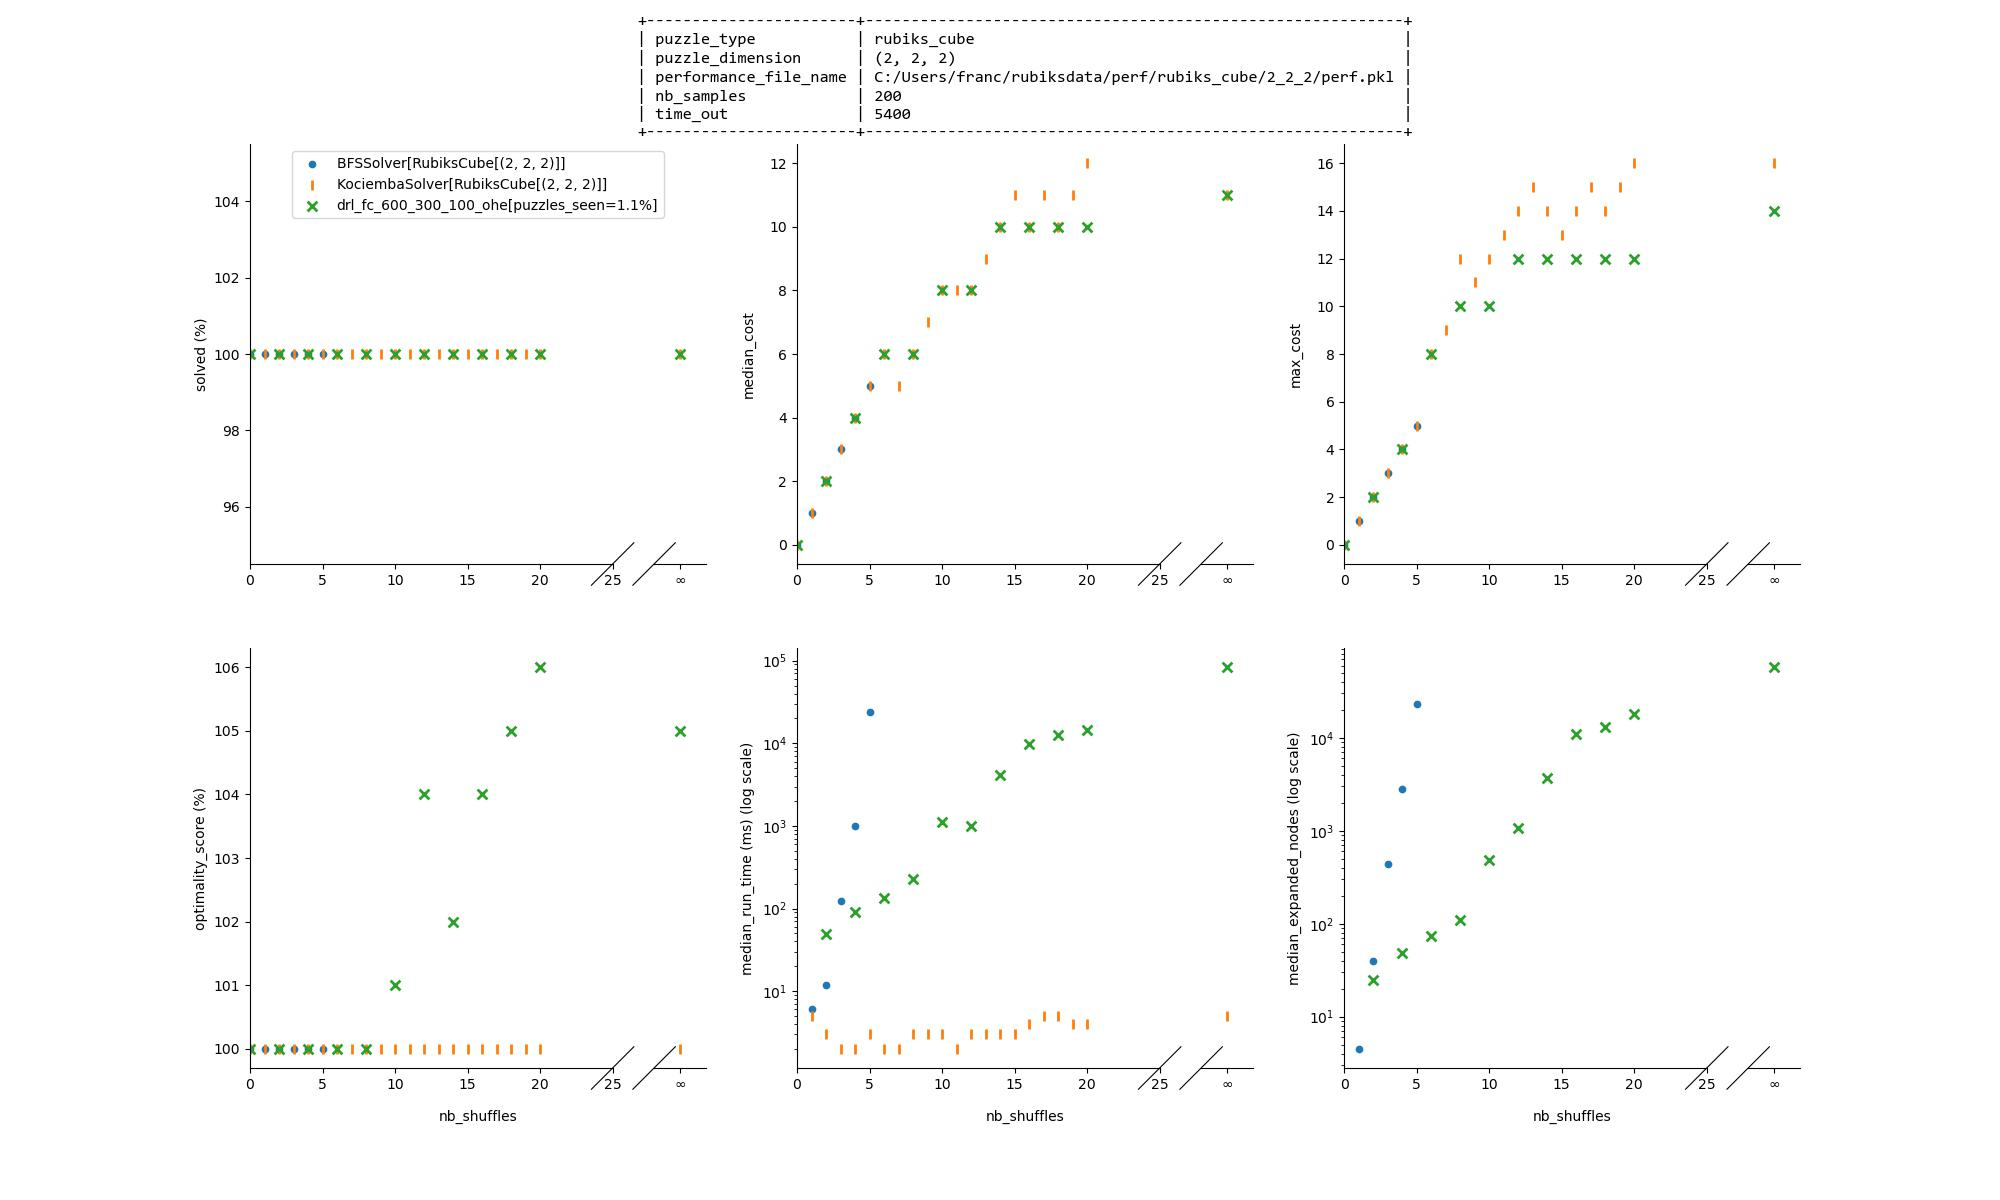
\includegraphics[scale=0.55]{./Figures/222RCPerformance}}
  \caption[222RCPerformance]{Solvers' performance comparison 2x2x2 \textbf{RC}}
  \label{fig:222RCPerformance}
\end{figure}



%-----------------------------------
%	SUBSECTION 1
%-----------------------------------
\Section{3x3x3}
\label{sec:ResRubiks333}

I did not get to run very many experiments on the 3x3x3 \textbf{RC}. The results of the performance test (50 random configurations for levels of difficulty from 2 to 40 by increment of 2 as well as $\infty$ shuffling) can be found on figure \ref{fig:333RCPerformance}.
\begin{itemize}
\item Here again, Kociemba does not show optimality, since we can see that my A$^{*}[Kociemba]$, that is A$^{*}$ using Kociemba as a heuristic, performs much better than Kociemba (solutions about 20\% shorter at $\infty$ shuffling). This is not surprising though since Kociemba 3x3x3 does not claim to be optimal and is meant to find solution in the 40 moves at most (which is what I have observed indeed). A$^{*}[Kociemba]$ never took more than 30 moves on any of the cubes presented to it, which is not bad given the known God number of 26 in the quarter-turn-metric (as discussed earlier in \ref{Theory:333RCSSS})
\item A$^{*}$[\textbf{DL}] managed to solve all puzzles scrambled less than 10 times, and found shorter worst case solutions than even A$^{*}[Kociemba]$ on which it was trained. Within the 2 hours time out, it failed to solve one of the 50 cubes for difficulty 10, and two of the 50 cubes of difficulty 12, so i did not try further than that.
\item A$^{*}$[\textbf{DRL}] only managed to solve all puzzles of difficulty less than 6 but at least did find only optimal solutions (compared with \textbf{BFS}).
\end{itemize}


\begin{figure}[H]
  \noindent
  \makebox[\textwidth]{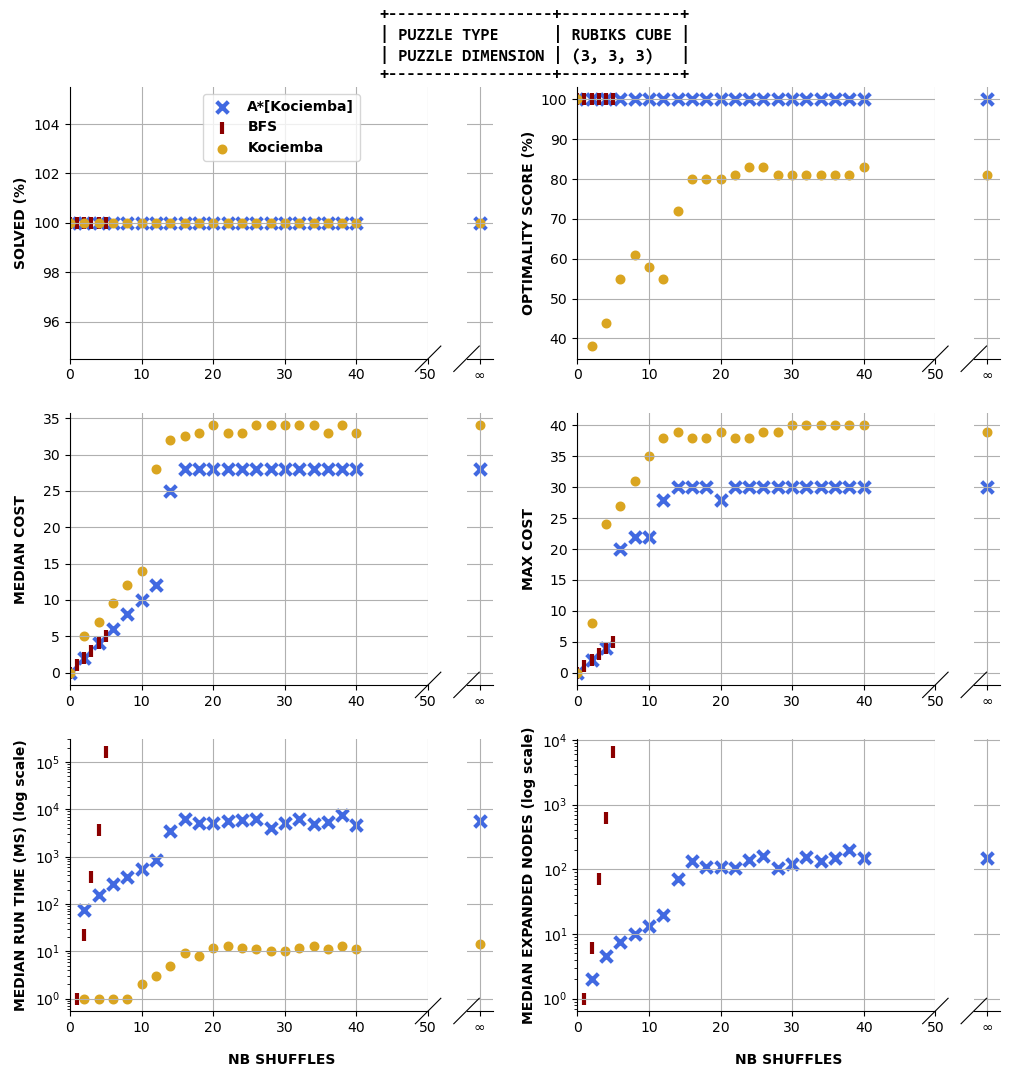
\includegraphics[scale=0.55]{./Figures/333RCPerformance}}
  \caption[333RCPerformance]{Solvers' performance comparison 3x3x3 \textbf{RC}}
  \label{fig:333RCPerformance}
\end{figure}
